\documentclass[10pt,a4paper]{article}
\usepackage[latin1]{inputenc}
\usepackage[spanish]{babel}
\usepackage{amsmath}
\usepackage{amsfonts}
\usepackage{amssymb}
\usepackage{graphicx}
\usepackage{textcomp}
\author{Santiago Videla - Francisco Javier Herrero}
\title{Pr\'actico Especial II: Selecci\'on de Distribuciones de Probabilidad}
\pagestyle{headings}
\begin{document}
\maketitle
\newpage
\tableofcontents
\newpage

\section{Independencia estad\'istica}

\paragraph{}
A partir de los datos obtenidos en la simulaci\'on, se corroboro la
independencia de los mismos mediante un \textit{scatter plot} como se puede ver
en la Figura~\ref{scatter}. Los valores observados, se distribuyen de manera
aleatoria en el primer cuadrante del plano, lo que indica la independencia de
los datos.

\begin{figure}
  \centering
  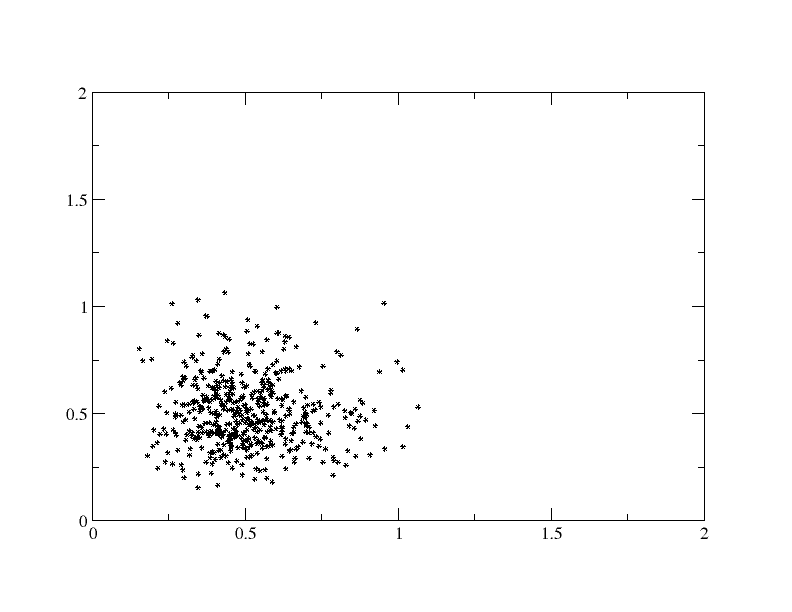
\includegraphics[scale=0.5]{scatter.png} 
  \caption{Scatter}
  \label{scatter}
\end{figure}

\section{Estad\'istica}

\begin{itemize}
  \item \textbf{M\'inimo:} 0.153672
  \item \textbf{M\'aximo:} 1.064818
  \item \textbf{Mediana:} 0.491458
  \item \textbf{Media:} 0.509307
  \item \textbf{1er. cuartil}: 0.398686
  \item \textbf{2do. cuartil}: 0.600152
  \item \textbf{Varianza:} 0.026880
  \item \textbf{Asimetria:} 0.652167
\end{itemize}

\begin{figure}
  \centering
  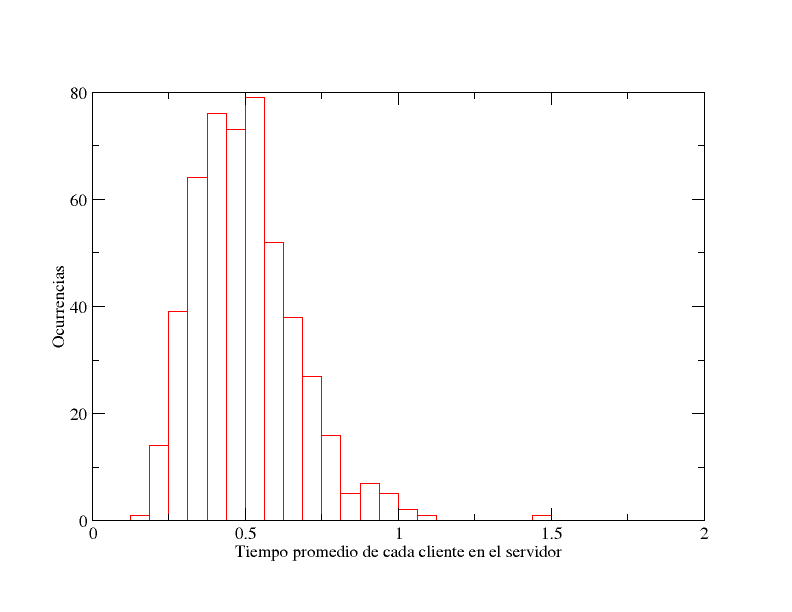
\includegraphics[scale=0.5]{histogram.png} 
  \caption{Histograma}
  \label{histogram}
\end{figure}

\begin{figure}
  \centering
  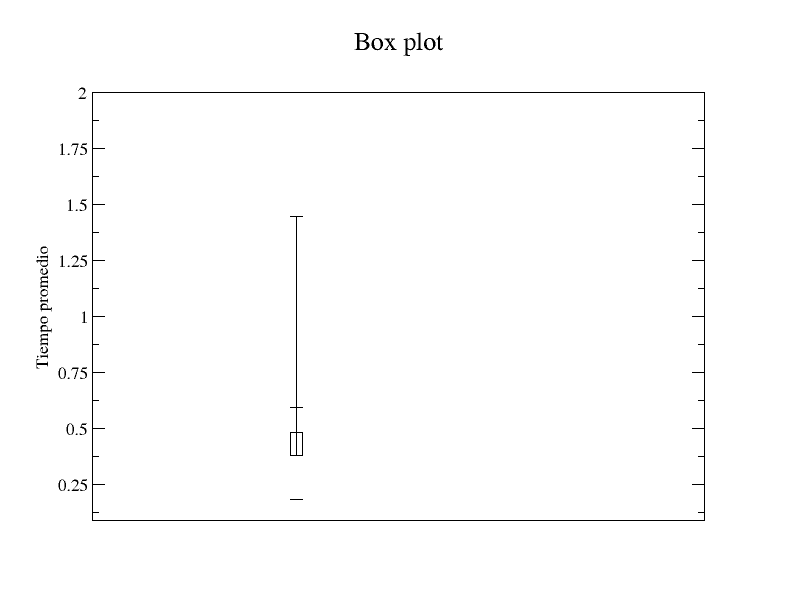
\includegraphics[scale=0.5]{boxplot.png} 
  \caption{Boxplot}
  \label{boxplot}
\end{figure}

\section{Estimacion de par\'ametros}

\begin{itemize}
  \item N($\mu$, $\sigma^{2}$): \\
    $\mu = 0.509307$ \\
    $\sigma^{2} = 0.026826$
  \item LN($\mu$, $\sigma^{2}$): \\
    $\mu = -0.727032$ \\
    $\sigma^{2} = 0.108136$
  \item Gamma($\alpha$, $\beta$): \\
    $\alpha = 9.789000$ \\
    $\beta = 0.052028$
\end{itemize}

\section{Bondad de los ajustes}

\begin{figure}
  \centering
  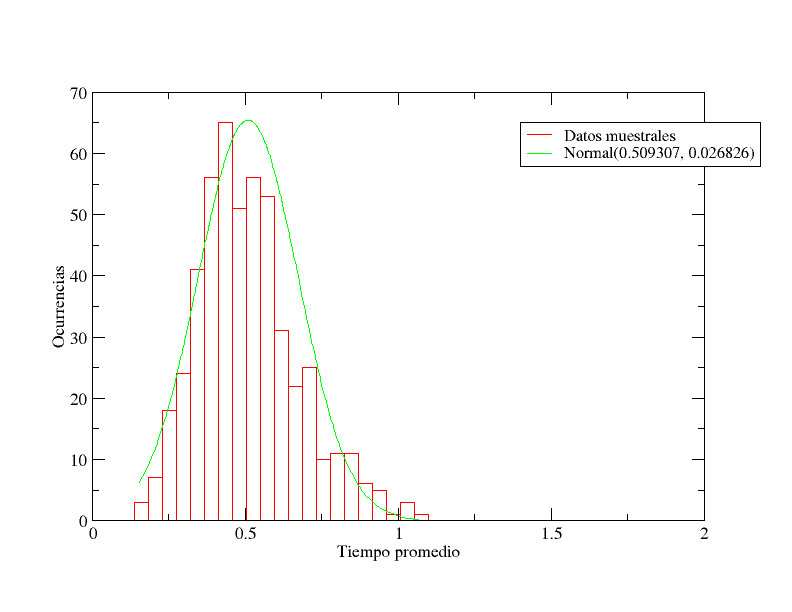
\includegraphics[scale=0.5]{freq-normal.png} 
  \caption{Muestra/Normal}
  \label{freq-normal}
\end{figure}

\begin{figure}
  \centering
  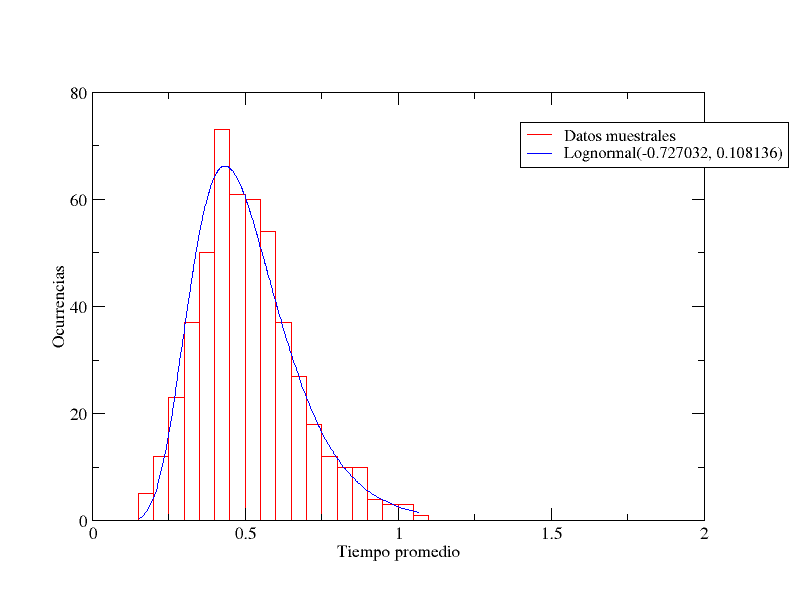
\includegraphics[scale=0.5]{freq-lognormal.png} 
  \caption{Muestra/LogNormal}
  \label{freq-lognormal}
\end{figure}

\begin{figure}
  \centering
  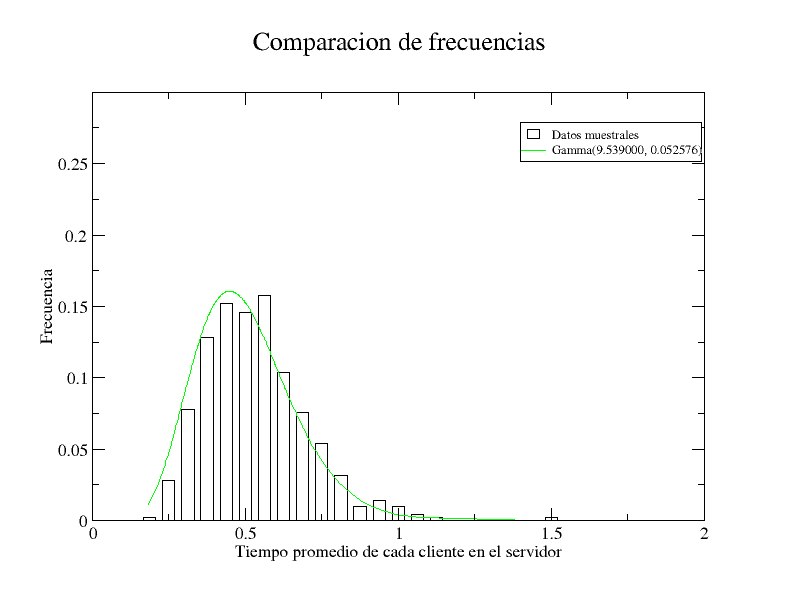
\includegraphics[scale=0.5]{freq-gamma.png} 
  \caption{Muestra/Gamma}
  \label{freq-gamma}
\end{figure}

\end{document}